\chapter{La Biología}
\label{biologia}

\epigraph{Essentially, all models are wrong,
but some are useful.}%
{\textbf{George E. P. Box}}

\par Dado a que el presente informe corresponde a un trabajo de Ciencias de la Computación, sólo se presentarán algunas definiciones y conceptos biológicos elementales que brindarán al lector la capacidad de comprender los temas abordados en los próximos capítulos, ya que se utilizará un lenguaje al cual el mismo puede no estar habituado. No se abordarán rigurosamente todos los conceptos biológicos involucrados, quedando como tarea del lector interesado.

\section{Introducción a la Biología}

\par La \emph{Biología} es una ciencia que tiene como objeto de estudio a los seres vivos. Se ocupa tanto de la descripción de las características y los comportamientos de los organismos individuales como de las especies en su conjunto, así como de la reproducción de los seres vivos y de las interacciones entre ellos y el entorno. De este modo, trata de estudiar la estructura y dinámica funcional comunes a todos los seres vivos, con el fin de establecer las leyes generales que rigen la vida orgánica y los principios explicativos fundamentales de la misma\cite{curtis}. 

\subsection{Niveles de Organización Biológica}
\par Los \emph{niveles de organización biológica} son eslabones organizados de forma jerárquica, es decir, están organizados desde lo más simple hasta lo más complejo. Estos niveles se utilizan para clasificar la materia, de acuerdo a su tamaño y/o cantidad. A continuación se detallan los diferentes niveles de organización biológica:

\begin{itemize}
	\item \textbf{Nivel Atómico:} constituido por átomos. Aquellos elementos
			que forman la materia viva se conocen con el nombre
			de \emph{bioelementos}. Dentro de los mismos se encuentran 
			el carbono, el hidrógeno, el oxígeno, el nitrógeno, el
			azufre y el fósforo.

	\item \textbf{Nivel Molecular:} este nivel está formado por las
			moléculas que se originan al unirse dos o más átomos.
			Las moléculas que constituyen la materia viva se
			denominan \emph{biomoléculas}. Éstas pueden ser
			inorgánicas como el agua, las sales minerales o los
			gases, u orgánicas como los glúcidos, los lípidos, las
			proteínas y los ácidos nucleicos.

	\item \textbf{Nivel Celular:} se incluyen las células. Una célula
			es la menor porción de materia viva que conforman los organismo, dentro de 
			la cual tienen lugar todas las funciones vitales. Toda célula está
			formada por los niveles inferiores, el molecular y el
			atómico. La complejidad de este nivel es mucho mayor,
			ya que la célula es una unidad anatómica y funcional,
			esto significa que es la estructura más pequeña que
			podría sobrevivir por si misma.

	\item \textbf{Nivel Pluricelular:} refiere a la asociación de varias
			células que pueden llegar a constituir un organismo
			completo. Este nivel se puede subdividir en los
			siguientes subniveles: \emph{tejidos}, \emph{órganos}, \emph{sistemas} y \emph{aparatos}.  
            En conjunto forman el individuo pluricelular.

	\item \textbf{Nivel Población:} incluye al conjunto de individuos de
			la misma especie que viven en un lugar concreto y en
			un tiempo determinado pudiendo relacionarse entre sí.

	\item \textbf{Nivel Ecosistema:} abarca las relaciones que se
			establecen entre las poblaciones que viven en un
			determinado lugar y el ambiente en el que habitan. 
\end{itemize}

\par Como se puede observar, la Biología abarca muchas áreas de estudio. El presente trabajo se encuentra a nivel molecular, por lo cual a continuación se desarrollarán conceptos pertinentes a este nivel, el cual es conocido dentro de la jerga como \textit{Biología Molecular}.

\subsection{Moléculas Orgánicas y Macromoléculas}
\label{molOrg}

\subsubsection{Moléculas Orgánicas}
Las moléculas orgánicas pueden definirse como aquellas que contienen carbono y se encuentran en los seres vivos. Hay dos tipos de moléculas orgánicas básicas:
\begin{enumerate}
    \item \textbf{Nucleótidos:} corresponden a pequeñas moléculas constituyentes de macromoléculas
    de mayor complejidad tales como los ácidos nucleicos. Un nucleótido está formado por un azúcar, un
    fosfato y una base nitrogenada como se observa en la figura~\ref{nucleotido}. Además de su papel en la
    formación de ácido nucleicos, tiene una función independiente y vital para la vida celular.
    Cuando un nucleótido se modifica por la unión de dos fosfatos, se convierte en un transportador de
    energía, la cual es necesaria para que se produzcan numerosas reacciones químicas celulares.

    Las bases nitrogenadas se clasifican en:
	\begin{itemize}
	    \item \textit{Bases nitrogenadas purínicas:} encontramos la Adenina(\textbf{A}) y Guanina(\textbf{G}).
		\item \textit{Bases nitrogenadas pirimidínicas:} encontramos la Timina(\textbf{T}), Citocina(\textbf{C}) y Uracilo(\textbf{U}).
		\item \textit{Bases nitrogenadas isoaloxacínicas:} encontramos la Flavina(\textbf{F}).
	\end{itemize}
	Las bases \textbf{A}, \textbf{G} y la \textbf{C} forman parte del DNA y RNA. La base \textbf{T} sólo forma parte del DNA, y en contrapartida, la base \textbf{U} sólo forma parte del RNA.	
    \begin{figure} [!h]       
    	    \hspace*{4cm}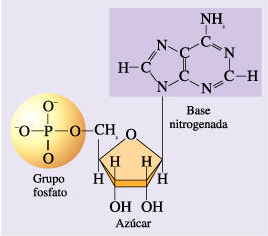
\includegraphics[width=2.5209in,height=2.000in]{image/nucleotido.png}
    		\caption{Estructura de un Nucleótido [4].}			
    		\label{nucleotido}
    \end{figure}				

    \item \textbf{Aminoácidos:} son las unidades estructurales que conforman las proteínas y sirven como materia prima para la formación de una gran variedad de compuestos nitrogenados con actividad fisiológica de vital importancia para la vida. Existen 20 aminoácidos que se exhiben en la figura~\ref{aminoac} y que  tienen codones específicos\footnote{Recordemos que un codón es un conjunto de tres nucleótidos.} en el código genético (figura ~\ref{codGen}). La unión de varios aminoácidos da lugar a cadenas llamadas polipéptidos o simplemente péptidos, que se denominan \emph{proteínas} cuando la cadena polipeptídica supera los 50 aminoácidos.
    	\begin{figure}[!h]
    		\hspace*{1cm}\begin{tabular}{| l | c | c |}
				\hline
				{\bf Nombre} & {\bf Ab. 3 letras} & {\bf Ab. 1 letra} \\
				\hline
				\hline
				Alanine (Alanina) & Ala & A\\\hline
				Arginine (Arginina) & Arg & R\\\hline
				Asparagine (Asparagina) & Asn & N\\\hline
				Aspartic acid (Aspartato) & Asp & D\\\hline
				Cytesine (Cisteína) & Cys & C\\\hline
				Glutamic acid (Ácido glutámico) & Glu & E\\\hline
				Glutamine (Glutamina) & Gln & Q\\\hline
				Glycine (Glicina) & Gly & G\\\hline
				Histidine (Histidina) & His & H\\\hline
				Isoleucine (Isoleucina) & Ile & I\\\hline
				Leucine (Leucina) & Leu & L\\\hline
				Lysine (Lisina) & Lys & K\\\hline
				Methionine (Metionina) & Met & M\\\hline
				Phenylalanine (Fenilalanina) & Phe & F\\\hline
				Proline (Prolina) & Pro & P\\\hline
				Serine (Serina) & Ser & S\\\hline
				Threonine (Treonina) & Thr & T\\\hline
				Tryptophan (Triptófano) & Trp & W\\\hline
				Tyrosine (Tirosina) & Tyr & Y\\\hline
				Valine (Valina) & Val & V\\\hline										
			\end{tabular}
			\caption{Tabla de representación de Aminoácidos [2].}
			\label{DnaRna}
			\label{aminoac}
		\end{figure}

		\begin{figure}[h]		
			\hspace*{2cm} 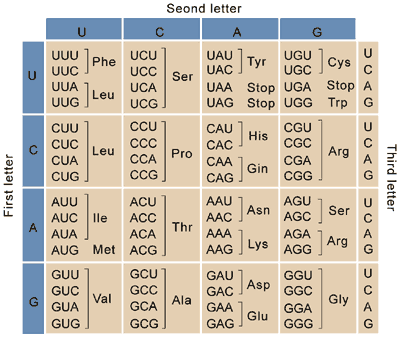
\includegraphics[width=3.9in, height=2.8in]{image/gencode.png}
			\caption{Código Genético [5].}
			\label{codGen}			
		\end{figure}	
\end{enumerate}

\vskip 2.5cm
\subsubsection{Macromoléculas}
Las macromoléculas son estructuras biológicas conformadas por un determinado número de moléculas orgánicas. Dentro de las macromoléculas podemos encontrar: \emph{Glúsidos}, \emph{Lípidos}, \emph{Proteínas} y
\emph{Ácidos Nucleicos}. Las dos primeros escapan al presente trabajo, por lo cual se deja a criterio del lector su investigación.

\begin{itemize}
	\item \textbf{Ácidos Nucleicos:} están conformados por secuencias de nucleótidos específicos, que son
    utilizados por todos los organismos para almacenar su información genética. La misma, está codificada
    mediante sucesivos codones, los cuales están conformados por tripletes de nucleótidos que codifican (traducen) a un determinado aminoácido. Existen dos tipos principales de ácidos nucleicos:
    	\begin{enumerate}
			\item \textbf{DNA (Ácido Desoxirribonucleico):} almacena y transmite la información    
			genética para el desarrollo y el funcionamiento de los organismos vivos y de algunos virus, la cual se hereda de generación en generación. Está formado por una doble cadena de nucleótidos, donde las dos hebras están unidas a través de las bases complementarias (respetando una estructura helicoidal) según el modelo propuesto por Watson\footnote{James Dewey Watson, biólogo estadounidense. Premio Nobel en Medicina.} y Crick\footnote{Francis Harry Compton Crick (1916-2004), físico, biólogo molecular y  neurocientífico británico. Premio Nobel en Medicina.} en 1953 (ver apéndice ~\ref{modelo}). El DNA contiene azúcares y fosfatos en su exterior y las bases en su interior. 
    		La doble hélice le proporciona al DNA una increíble estabilidad y permanencia. Las dos cadenas polinucleótidas se disponen en direcciones opuestas, es decir son antiparalelas, lo que significa que el extremo denominado \emph{5'} de una cadena se ubica en oposición al extremo denominado \emph{3'} de la otra cadena, tal como se exhibe en la figura~\ref{extremos}.

    		\begin{figure} [h]
				\begin{center}
					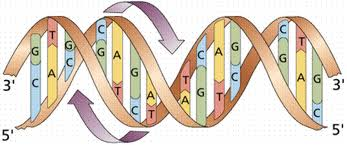
\includegraphics[width=2.9209in,height=1.0000in]{image/extremos.jpg}
					\caption{DNA: cadenas antiparalelas [6].}				
					\label{extremos}
				\end{center}
			\end{figure}	

			\item \textbf{RNA (Ácido Ribonucleico):} consiste en una hebra de cadena simple, la cual usualmente es trascripta a partir de una porción de DNA y se utiliza posteriormente en la célula para la síntesis de proteínas (sección~\ref{sintesisProteica}).			
		\end{enumerate}				
	Aunque el DNA y RNA son muy semejantes, desempeñan papeles biológicos muy diferentes. El DNA es el constituyente principal de los cromosomas de las células y es el portador del mensaje genético. En cambio, en RNA tiene como función transcribir el mensaje presente en el DNA y traducirlo a las proteínas. 
    Además, el DNA se encuentra principalmente en el núcleo celular, mientras que el RNA se encuentra en el citoplasma, donde se produce la síntesis de proteínas.							
	Otra diferencia entre estos dos tipos de ácidos nucleicos radica en las propias diferencias naturales existentes entre sus nucleótidos y residen en el tipo azúcar (ribosa en el caso del RNA y desoxirribosa en el caso del DNA) y las bases nitrogenadas características de cada uno.
	Otro rasgo a destacar, es que a pesar de que en la mayoría de las especies el DNA lleva la información genética, existen casos donde el RNA sirve como material genético (por ejemplo algunos virus tales como el TMV\footnote{Virus del mosaico del tabaco.}). En la figura~\ref{DnaRna} se puede observar gráficamente la cadena doble característica del DNA (parte derecha de la figura) y la cadena simple del RNA (parte izquierda de la figura).	
					
	\begin{figure} [h]
		\begin{center}
		   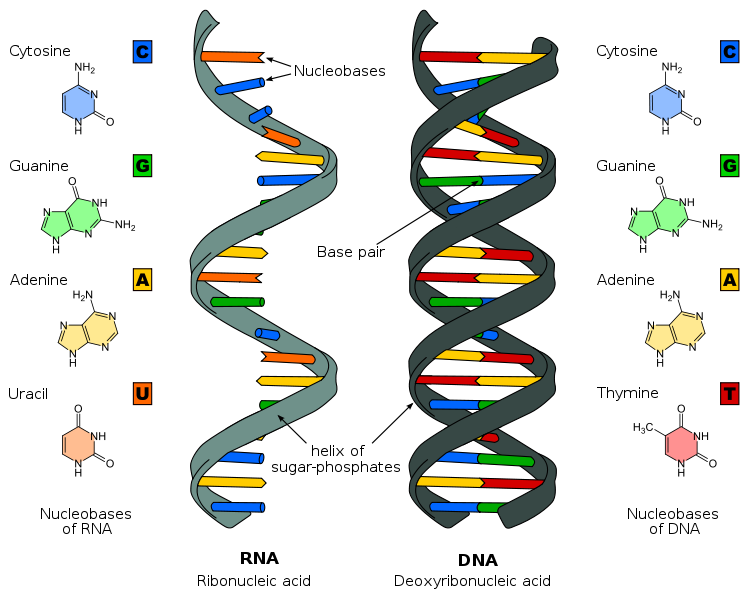
\includegraphics[width=5.0209in,height=4.0000in]{image/ARN-ADN.png}
		   \caption{Representación gráfica del RNA y DNA [7].}			
		   \label{DnaRna}
		\end{center}
	\end{figure}	

	\item \textbf{Proteínas:} son las moléculas más abundantes y de máxima importancia biológica porque la ordenación de los distintos monómeros\footnote{Un monómero es una molécula de pequeña masa muscular que unida a otros monómeros por medio de enlaces químicos forman macromoléculas denominadas \emph{polímeros}.} en su estructura permite que sean utilizados como vehículo de la información celular.
	Están formadas por secuencias de aminoácidos específicas (se considera proteína a aquellas cadenas de aminoácidos enlazados cuyo peso molecular es superior a 6000 Daltons), que adoptan una conformación tridimensional determinada debido a las interacciones electrostáticas existentes entre los residuos de sus aminoácidos constituyentes. 
	La estructura molecular de las proteínas (figura~\ref{proteina}) tiene varios niveles de organización, al igual que los ácidos nucleicos. La \textit{estructura primaria} consiste en una secuencia de aminoácido.
    A través de las interacciones entre los aminoácidos vecinos, una cadena polipeptídica se pliega y se enrosca para formar una \textit{estructura secundaria}. Las estructuras secundarias interactúan y se pliegan adicionalmente para forma lo que se conoce como \textit{estructura terciaria}, que es la forma completa, tridimensional de la proteína. Finalmente, algunas proteínas consisten en dos o más cadenas polipeptídicas que se asocian para producir una \textit{estructura cuaternaria.} 
	\par Las proteínas no son capaces de portar información genética y transmitirla a la descendencia, como ya se mencionó, este papel es realizado por los ácidos nucleicos, en particular por el DNA. Éste necesita de las proteínas para replicarse, y a su vez, las proteínas necesitan de la información que provee el DNA su síntesis.					
	\par Desde el punto de vista funcional, juegan un rol fundamental, dado que todo proceso biológico
	depende de la presencia y/o actividad de estas sustancias. Son proteínas casi todas las \textit{enzimas}
	(catalizadores de reacciones químicas en los organismos), \textit{hormonas} (reguladores de actividades celulares), \textit{hemoglobina} (transporte de sangre), \textit{anticuerpos} (encargados de acciones de defensa natural contra infecciones o agentes extraños), entre otras.
	\par Cabe destacar que existe una relación colineal con los genes\footnote{Un gen se define como un factor hereditario que determina una característica.}, es decir, hay una correspondencia directa entre la secuencia de nucleótidos del DNA y la secuencia de aminoácidos de una proteína. El concepto de colinealidad sugiere que el número de nucleótidos de un gen debería ser proporcional al número de aminoácidos de la proteína codificada por ese gen.

    \begin{figure} [h]
	    \begin{center}
		    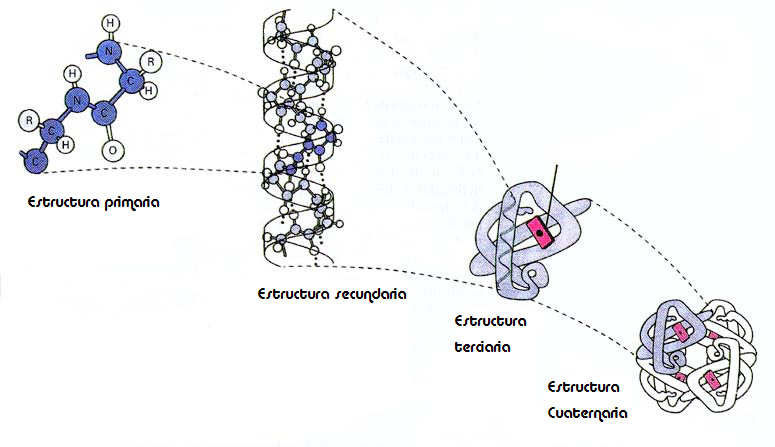
\includegraphics[width=5.7209in,height=2.7000in]{image/estructuraProteina.png}
		    \caption{Estructura molecular de las proteínas [8].}
		    \label{proteina}
	    \end{center}
    \end{figure}	
\end{itemize}

Las primeras investigaciones a cerca del material genético y su relación con DNA y proteínas mostraron que un cromosoma\footnote{Se denomina cromosoma a cada uno de los pequeños cuerpos en forma de bastoncillos en que se organiza la cromatina del núcleo celular durante las divisiones celulares. La cromatina es el conjunto de DNA y proteínas que se encuentra en el núcleo de las células.} estaba formado por DNA y proteínas en cantidades aproximadamente iguales. Por lo cual, ambos eran candidatos para desempeñar el papel de material genético. Las proteínas parecían ser la opción correcta dada su mayor complejidad química, aunque esta hipótesis era lógica fue errónea. 
El descubrimiento de la sustancia que puede transmitir características genéticas de una célula a otra resultó de los estudios con neumococos\footnote{Bacterias que causan la neumonía.}\cite{curtis}.

\subsection{Estructura del DNA}
\begin{itemize}
	\item \emph{Estructura Primaria}: consiste en una cadena de nucleótidos unidos entre sí por uniones fosfodiéster. 
	\item \emph{Estructura Secundaria}: se relaciona con su configuración tridimensional (su 		
				estructura helicoidal básica). Esta estructura puede adquirir diversas configuraciones de acuerdo con su secuencia de bases y las condiciones en que
				se encuentran.
				Dentro de las mismas, encontramos la estructura \textbf{B-DNA}, la cual depende de que la molécula esté rodeada por abundante agua, además es la estructura más estable. Por otro lado, la estructura \textbf{A-DNA} la cual se presenta cuando la cantidad de agua es menor. Y por último, la estructura \textbf{Z-DNA} la cual se genera cuando
				el DNA es colocado en una solución de alta concentración salina. Las estructuras mencionadas se exhiben en la figura~\ref{estrucDNA}.
\end{itemize}

\begin{figure} [h]
  		\hspace*{2cm}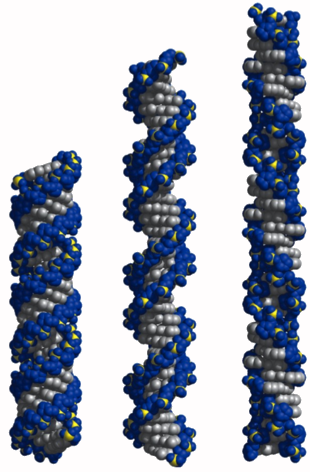
\includegraphics[width=3.5209in,height=3.5000in]{image/estructuraSecDNA.png}
   		\caption{Estructuras secundarias del DNA. A-DNA, B-DNA y Z-DNA de izquierda a derecha respectivamente [9].}
   		\label{estrucDNA}
\end{figure}	

\subsection{Replicación de DNA}
\par Consiste en el proceso a través del cual una célula duplica su DNA antes de dividirse. Dicho proceso es muy complejo, tal es así, que un componente defectuoso puede producir síntomas patológicos graves. 
\par La replicación es fundamental para el funcionamiento y mantenimiento de la célula y ocurre sólo una vez en cada generación celular, resultando esencial en la duplicación de los cromosomas.

\vskip 0.5cm
\noindent \textbf{Replicación semicorservativa}
\vskip 0.025cm

Básicamente la molécula de DNA se abre por el medio, separándose por bases apareadas (A=T; C=G) al nivel de los puentes de hidrógeno. A medida que las dos cadenas se separan, actúan como moldes o guías, es decir, cada una dirige la síntesis de una nueva cadena complementaria, utilizando las materias primas de la célula (figura~\ref{semi}).
Este modelo de replicación se conoce como \textit{replicación semiconservadora}, dado que se conserva la mitad de la molécula original en cada nueva cadena hija. Esto es, si hay una \textbf{T} presente en la cadena original, solamente puede ubicarse una \textbf{A} en el lugar correspondiente en la nueva cadena, de igual forma, una \textbf{G} sólo se apareará con una \textbf{C}, y así sucesivamente. Así, cada cadena forma una copia de su cadena complementaria original y se producen dos réplicas exactas de la molécula.

\begin{figure} [h]
		\hspace*{4.5cm}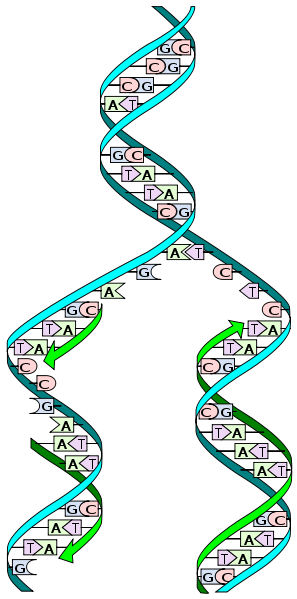
\includegraphics[width=2.1209in,height=3.5000in]{image/replicacionSemiconservativa2.png}
		\caption{Replicación semiconservativa [10].}		
		\label{semi}
\end{figure}				

El proceso real de replicación en un poco más complejo que la replicación semiconservadora. La replicación del DNA requiere de diferentes enzimas, las cuales catalizan un paso particular del proceso. 

\subsection{Del DNA a la Proteína}
\subsubsection{El Dogma Central de la Biología}
\par Este dogma\footnote{Un dogma es una proposición que se asigna como cierta e innegable, no sujeta a prueba de veracidad.} proclamado por Francis Crick en 1956 indica que la información fluye en una única dirección, es decir, el DNA transfiere la información al RNA, el cual controla directamente la síntesis de proteínas (figura ~\ref{dogma}). Así, el genotipo\footnote{El genotipo es la totalidad de la información genética que posee un organismo en particular, en forma de DNA. También puede definirse como el conjunto de genes de un organismo.} determina el fenotipo\footnote{Se denomina fenotipo a la expresión del genotipo en función de un determinado ambiente. También puede definirse como el conjunto de rasgos de un organismo.}, dictando la composición de las proteínas. Sin embargo, estas últimas no alteran al genotipo, es decir, las proteínas no envían instrucciones de regreso. 
\par Este dogma posee algunas excepciones, la principal de ellas es el proceso conocido como \textit{transcripción inversa}, en el cual la información codificada por cierto virus que contienen RNA se transcribe al DNA por la acción de la enzima transcriptasa inversa. 
\par El hecho de que la información fluya del DNA al RNA, y de éste a las proteínas suministró cierta confirmación de la teoría darwinista de la evolución. Según esta teoría, la selección natural actúa sobre las variaciones heredables encontradas en el DNA\cite{curtis}.

\begin{figure} [h]
	\hspace*{3cm}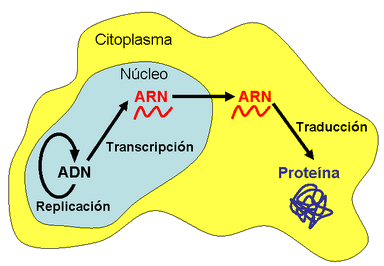
\includegraphics[width=3.1209in,height=1.4000in]{image/rel.png} 
	\caption{El Dogma Central [11].}	
	\label{dogma}
\end{figure}				

Existen diferentes clases de RNA que desempeñan diferentes funciones como intermediarios entre los pasos que llevan del DNA a las proteínas. Éstos son:
\begin{itemize}
	\item RNA mensajero\textbf{($_m$RNA):} se encuentra tanto en el núcleo como en el citoplasma de una célula. Su función es portar el código genético para las proteínas, es decir, transportan las instrucciones de codificación de las proteínas desde el DNA hasta el ribosoma. Después de unirse al ribosoma, una molécula de $_m$RNA especifica la secuencia de los aminoácidos de la proteína y proporciona un molde para unirlos.
	\item RNA de transferencia\textbf{($_t$RNA):} se encuentra sólo en el citoplasma. Sirve como enlace entre la secuencia codificante de nucleótidos de $_m$RNA y la secuencia de aminoácidos de una cadena polipeptídica. Cada $_t$RNA se une a un tipo particular de aminoácido y ayuda a incorporarlo a una cadena polipeptídica.
	\item RNA ribosómico\textbf{($_r$RNA):} se encuentra sólo en el citoplasma. Es un componente estructural y funcional del ribosoma (sitio de ensamblaje de proteínas).
	\item RNA interferente pequeño\textbf{($_s$$_i$RNA)} y microRNA\textbf{($_m$$_i$RNA)}: son moléculas muy pequeñas presentes en las células eucariotas que inhiben específicamente la expresión de genes a nivel post-transcripcional, en respuesta a la presencia de RNA de doble hebra que proviene de la propia célula ($_m$$_i$RNA) o del exterior de la misma (RNA pequeños de interferencia o $_s$$_i$RNA). Particularmente, los $_m$$_i$RNA son pequeños RNA codificados en el DNA de las distintas especies que regulan la expresión de una gran fracción de las proteínas. Para que esto ocurra, el debe encontrar nucleótidos complementarios (la unión se ve favorecida si estos nucleótidos no se ven comprometidos en la estructura secundario de la molécula) en el $_m$RNA blanco. %Recientemente se ha demostrado que, no sólo la unión de los $_m$$_i$RNA a la región no codificante puede disminuir la expresión proteica, sino que se han registrado uniones a regiones codificantes que producen una regulación negativa.
\end{itemize}

\subsubsection{Transcripción}
En este proceso las secuencias de DNA son copiadas a RNA mediante una enzima llamada RNA polimerasa. Dicha enzima sintetiza un RNA que mantiene la información de la secuencia del DNA. De esta manera, la transcripción del DNA tambiFén podría llamarse síntesis del RNA. En términos generales es la síntesis de una molécula de RNA a partir de un molde de DNA.

La transcripción es un proceso muy parecido a la replicación del DNA pero existe una diferencia fundamental relacionada con la longitud del molde empleado. Durante la replicación se copian todos los nucleótidos del molde de DNA pero durante la transcripción sólo pequeñas porciones de DNA se transcriben a RNA (casi siempre un único gen o a lo sumo algunos genes). Por lo cual, la transcripción es un proceso selectivo, es decir, se transcriben genes individuales sólo cuando se requieren sus productos. Esta selectividad implica la identificación de genes individuales y su transcripción en el momento y lugar adecuado.

\par Las moléculas de RNA son largas copias de secuencias de una cadena simple de DNA pero, a diferencia de las moléculas de DNA, se encuentran en su mayoría como moléculas de cadena única. Cada nueva molécula de RNA se copia de una de las dos cadenas de DNA (la cadena molde, la otra cadena restante de la doble hélice en general no se transcribe) según el mismo principio de apareamiento de bases que gobierna la replicación del DNA, como se puede observar en la figura~\ref{transcripcion}. 

\begin{figure} [h]
	\hspace*{3.5cm}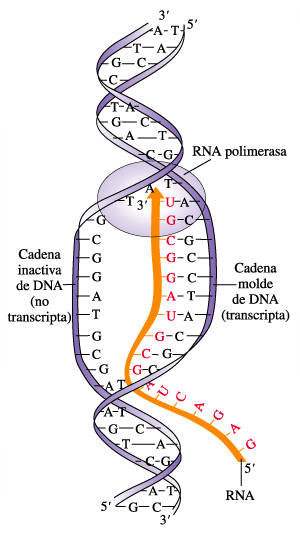
\includegraphics[width=2.2209in,height=3.5000in]{image/transcripcion.jpg}
	\caption{Representación esquemática de la transcripción del RNA [12].}
	\label{transcripcion}
\end{figure}				

\par La mayor parte de los transcriptos sufren un procedimiento posterior a la transcripción antes de dejar el núcleo e ingresar al citoplasma llamado \textit{splicing}.
\par En conclusión, el RNA transcripto a partir del DNA es la copia activa de la información genética.


\subsubsection{Traducción} 
\label{sintesisProteica}
En términos generales, el proceso consiste en tomar la información codificada en el DNA y transcripta en el RNA y traducirla a una cadena polipeptídica.
En este proceso entran en juego además del $_m$RNA, el $_r$RNA y $_t$RNA, los cuales se transcriben a partir de la cadena molde de DNA de la misma manera que el RNA.

Las moléculas de $_t$RNA  son el diccionario por medio del cual se traduce el lenguaje de los ácidos nucleicos al lenguaje de las proteínas. Cada molécula de $_t$RNA  tiene dos sitios de unión importantes como se observa en la Figura~\ref{ARNt}. Uno de ellos, conocido como el \textit{anticodón}, se acopla al codón de la molécula de RNA. El otro, en el extremo 3' de la molécula de $_t$RNA, se acopla a un aminoácido particular. Así, el $_t$RNA  permite que los aminoácidos se alineen de acuerdo con la secuencia de nucleótidos en el $_m$RNA.
\par Todas las moléculas de $_t$RNA  presentan una estructura tridimensional (estructura secundaria) similar a la hoja de trébol con regiones de la molécula formando doble cadena como se puede observar en la figura~\ref{ARNt}. En el extremo 3' de la molécula se acopla al aminoácido. (siempre termina en una secuencia (5')-CCA-(3')).

\begin{figure} [h]
	\hspace*{4cm}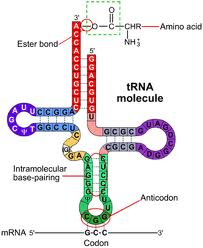
\includegraphics[width=2.2209in,height=2.0000in]{image/rnat1.jpg}
	\caption{Modelo de la estructura de una molécula de $_t$RNA [13].}	
	\label{ARNt}
\end{figure}		

La síntesis de proteínas se conoce también como \textbf{traducción}, dado que es la transferencia de información del lenguaje de los nucleótidos al de los aminoácidos. Este proceso ocurre en tres etapas: iniciación, elongación y terminación. Las mismas se dejan a criterio del lector.

\subsubsection{Excepciones al Dogma} 

\par Como se puede observar en la figura~\ref{excepcionesDogma}, existen dos excepciones al dogma conocidas como \textit{transcriptasa inversa o transcripción inversa} y \textit{replicación del RNA}.
\par La transcripción inversa\cite{curtis} es el proceso que consiste en la transferencia de información desde el RNA a la molécula de DNA y tiene lugar en los retrovirus\footnote{Un retrovirus es un virus RNA que se duplica en una célula huésped utilizando la transcriptasa inversa.}.
\par La replicación de RNA\cite{curtis} es el proceso que consiste en sintetizar RNA a partir de RNA y tiene lugar en algunos virus con genoma RNA (ejemplo TMV).
\par Los mecanismos mencionados escapan a este trabajo, por lo cual se deja a criterio del lector profundizar en éstos conceptos.
\begin{figure} [h]
	\hspace*{2cm}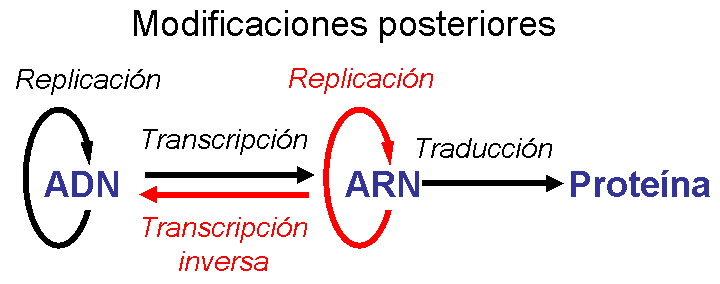
\includegraphics[width=3.8209in,height=0.9000in]{image/excepcionesDogma.jpg}
	\caption{Excepciones al Dogma Central [14].}
	\label{excepcionesDogma}
\end{figure}	

\vskip 1cm
\section{Estructura Secundaria del RNA} 
La estructura de una molécula de RNA se divide en tres niveles fundamentales de organización: primario, secundario y terciario. En particular, en este trabajo nos interesa el nivel secundario, por lo cual a continuación se abordará dicho nivel.

\par En términos generales, el plegamiento de una secuencia de RNA entre sus bases complementarias determina lo que se denomina \emph{Estructura Secundaria de RNA}. Conocer la estructura secundaria es fundamental para comprender el funcionamiento de los distintos tipos de RNA y de la célula en general. 

\par Más formalmente, dada una estructura primaria o secuencia de RNA de longitud $n$, la estructura secundaria es un conjunto S de pares $(i,j)$ con $1\leq i < j \leq n$ tal que para todo, $(i,j), (i',j') \in S$ se satisfacen las tres siguientes     condiciones:
\begin{itemize}
	\item $j-i > 3$
    \item $i=i' \Leftrightarrow j=j'$
    \item $i< i'\Rightarrow i < i' < j' < j \lor i < j < i' < j'$ 
\end{itemize}

\subsection{Predicción de la Estructura Secundaria (\textbf{\emph{folding}})}

\par El \emph{folding} o predicción de la estructura secundaria corresponde a un conjunto de técnicas bioinformáticas cuyo objetivo es predecir la estructura secundaria de una secuencia de RNA o de una proteína, basándose sólo en el conocimiento de su estructura primaria (secuencia de nucleótidos o de aminoácidos, respectivamente). Se da el caso en que diferentes secuencias de RNA pueden tener la misma estructura secundaria, por lo que también interesa determinar para una estructura secundaria dada, las secuencias de RNA que conservan esa estructura.

\par La existencia de una asociación entre la secuencia de aminoácidos y secuencia de nucleótidos respecto de la estructura secundaria adoptada en la proteína y el RNA respectivamente es la hipótesis fundamental sobre la cual están basados todos los métodos de predicción de estructura secundaria. 
 
\par En inglés, se suele denominar a la predicción de estructuras secundarias como \emph{folding} e \emph{inverse folding} al reconocimiento de posibles secuencias que conservan una estructura secundaria determinada. \emph{Inverse folding} escapa a este trabajo, pero puede obtenerse mayor información consultando el proyecto \textbf{vac-o}\footnote{\url{vac-o.googecode.com}}.

\par Esencialmente existen 2 tipos de algoritmos para determinar o predecir la estructura secundaria de una secuencia de RNA.
\begin{itemize} 
	\item \textbf{Predicción por mfe (Minimal Free Energy)}: propuesto e implementado por Michael Zuker en 1981\cite{Zuker81}, utiliza programación dinámica para encontrar la estructura secundaria que minimiza la energía libre.

	\item \textbf{Predicción comparativa}: utiliza diferentes métodos para comparar secuencias y estructuras con el fin de obtener una estructura por ``consenso''\cite{Gardner04}.
\end{itemize}

Si bien la ``predicción comparativa'' presenta un incremento en la fidelidad de los resultados obtenidos con respecto a la ``predicción por mfe'', este tipo de algoritmos requieren la existencia de un conjunto de secuencias relacionadas entre sí (homólogas) y no siempre es posible obtenerlas. En particular, para este trabajo interesa poder conocer la estructura secundaria de una sola secuencia, por lo que la ``predicción comparativa'' fue descartada.

\par Entre las implementaciones de la ``predicción por mfe'' se destacan \textbf{UNAFold}\cite{unafold} y \textbf{RNAfold}\cite{Hofacker94}. Ambas implementan el algoritmo propuesto por Michael Zuker con complejidad $\mathcal{O}(N^{3})$ donde $N$ es la longitud de la secuencia. En el capítulo ~\ref{analisis} se detallarán brevemente las implementaciones mencionadas.

\subsection{RNA Motifs}
\label{RNAmotifs}
El término ``Motifs''\cite{motifs}, también conocido como \emph{elementos regulatorios o sitios de unión} representa los diversos bloques que conforman una estructura secundaria de RNA. Juegan un papel funcional en la formación de la estructura terciaria y pueden estar sujetos a restricciones evolutivas. Dentro de estos bloques se encuentran:

\begin{itemize}

\item \emph{Single strand}: corresponde a un nucleótido no apareado (figura~\ref{motifs}.a).

\item \emph{Helices-Dúplex}: más de la mitad de los nucleótidos están presentes en las \emph{hélices} de doble cadena. Las regiones \emph{dúplex} pueden formar largas interacciones, las cuales son cruciales para determinar y estabilizar el pliegue global de una molécula de RNA. Los dúplex de RNA no son uniformes, aunque su variabilidad es menor que en el DNA. Estas variaciones dependen de la secuencia y el contexto estructural de la hélice con respecto al contexto global de la estructura tridimensional. (figuras~\ref{motifs}.b y~\ref{motifs}.c).

\item \emph{Bulges:} se forman cuando un tracto de la doble hélice se separa por uno o más nucleótidos no apareados. (figuras~\ref{motifs}.d y~\ref{motifs}.e).

\item \emph{Hairpins}: corresponde al elemento más común de una estructura secundaria y varían de 2 a 14 nucleótidos. Se forma cuando las secuencias nucleótidos de una misma cadena son estructuras complementarias invertidas.
Un \emph{hairpin} consiste de una región de bases apareadas (\emph{tallo}) y, a veces, incluye bases ``no apareadas'' intermedias (\emph{bucle}). Cuando las estructuras complementarias son contiguas, el hairpin presenta un tallo pero no un bucle. Los pequeño hairpin loop contienen un alto grado de estructura, mientras que los más largos (aquellos que contienen más de 7 u 8 nucleótidos no apareados) generalmente no están bien estructurados y termodinámicamente son menos estables. (figura~\ref{motifs}.f)
    
\item \emph{Internal Loop}: se forman cuando los dos tractos de la doble hélice se separan por uno o más nucleótidos no apareados. Los \emph{internal loop} puede ser simétricos o asimétricos, dependiendo del número de bases que contega cada cadena. (figuras~\ref{motifs}.g y~\ref{motifs}.h y~\ref{motifs}.i)

\item \emph{Multi-Loop}: se forma por la intersección de dos o más dobles hélices. Estas dobles hélices se separan por secuencias de cero o más nucleótidos no apareados. (figura~\ref{motifs}.j)

\item \emph{External Loop}: motif inicial de una estructura (figura~\ref{motifs}.k) 

\end{itemize}
\par Las moléculas de RNA pueden contener numerosos motifs, lo que les permite plegarse y formar estructuras muy complejas tal como se puede observar en la figura~\ref{compleja}.

\vskip 10cm
\begin{figure} [!h]
	\begin{center}
		\vskip 2cm
		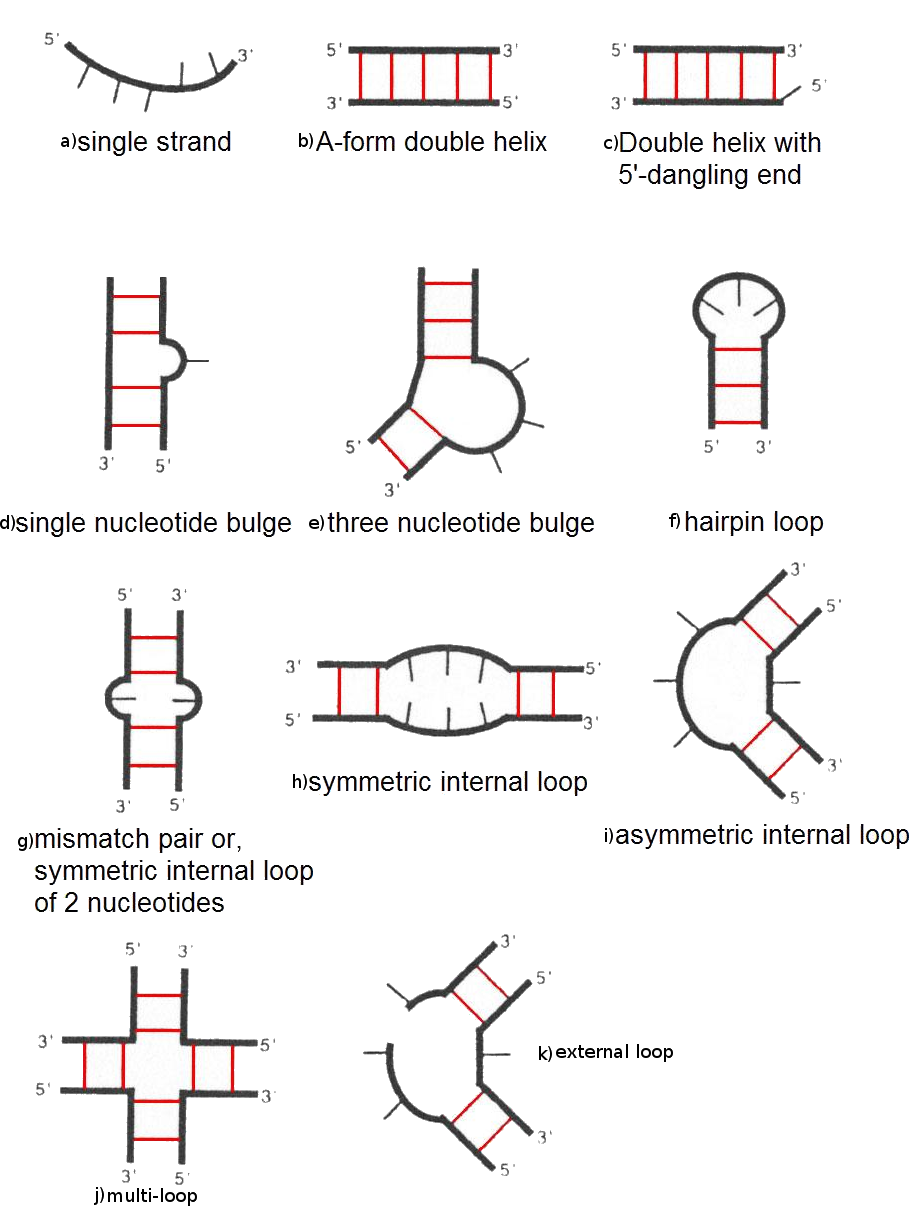
\includegraphics[width=5.5209in,height=5.3000in]{image/motifs2.png}
		\caption{RNA Motifs [2].}
		\label{motifs}
	\end{center}
\end{figure}

\begin{figure} [h]	
		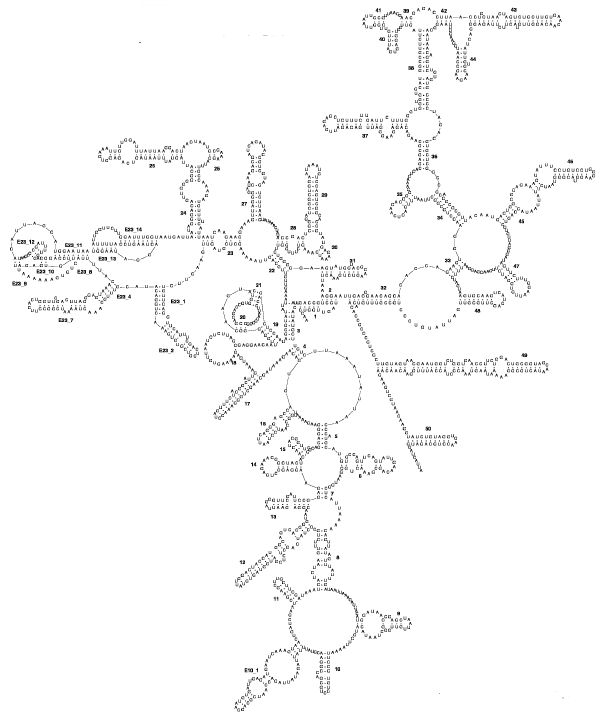
\includegraphics[width=5.8209in,height=5.2000in]{image/compleja.png}
		\caption{Estructura Secundaria Compleja [15].}		
		\label{compleja}	
\end{figure}	


\vskip 15cm
\section{Hibridación}
\par El fenómeno de apareamiento de bases (bases complementarias: A-T y C-G) para formar una doble hélice se llama \emph{hibridación}, dado que puede utilizarse para formar DNA híbrido compuesto por cadenas de diferentes orígenes tal como se exhibe en la figura ~\ref{hibridacion}.

\par Este proceso ocurre en solución y requiere de ciertos factores, tales como, un determinado pH, determinada temperatura, cierta concentración de sales, etcétera. Dependiendo de estas condiciones, es posible que en los híbridos existan malos apareamientos (A-C, por ejemplo).

\par El origen de cada una de las hebras es irrelevante, sólo importa la secuencia (que un número significativo de bases sea complementario entre las dos).

\begin{figure}[h!]
	\centering
		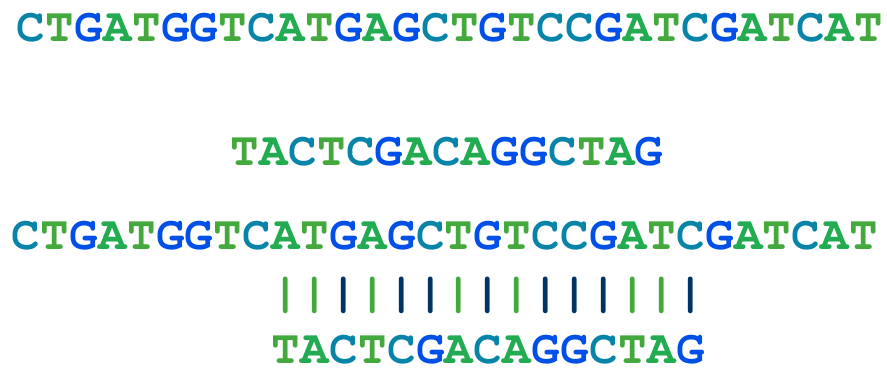
\includegraphics[scale=0.27]{image/hibridacion.png}
	\caption{Hibridación [2].}
	\label{hibridacion} 
\end{figure} 

\section{Energía Libre y Estabilidad} 
\par El concepto de ``Energía Libre'' hace referencia al total de energía contenida en un sistema que está disponible para realizar trabajo, como por ejemplo una molécula de RNA con una estructura secundaria, la cual le permite al mismo realizar trabajo. Una molécula de RNA puede estar dotada de una cierta cantidad de energía libre mediante interacciones eléctricas no neutralizadas en su estructura primaria, por lo tanto, esta energía se utilizará para plegar la misma hacia una estructura secundaria más estable. De este modo, un RNA con una estructura secundaria estable, implica una molécula en la cual sus interacciones eléctricas entre nucleótidos se hallan completamente neutralizadas. 
\par Este concepto es muy complejo e involucra nociones básicas de termodinámica, por lo cual su abordaje escapa al presente trabajo de ciencias de la computación, por lo cual puede indagarse más al respecto en \cite{energialibre}. 

\par La termodinámica de las interacciones RNA-RNA \\
\cite{freeEnergy} puede ser entendida como la suma de dos contribuciones de energía:
\begin{center}
	$\Delta$G = $\Delta$G$_u$ + $\Delta$G$_h$ 
\end{center}
donde:
\begin{itemize}
	\item $\Delta$G: energía libre.
	\item $\Delta$G$_u$: energía necesaria para exponer el sitio de unión para una interacción. 
	\item $\Delta$G$_h$: energía obtenida a partir de hibridación en el sitio de unión.
\end{itemize}